\chapter{Medir y comparar con YOLO26n}
\label{cap:evaluar}

\begin{enpocas}
Cómo se calcula el mAP, por qué hay que medir todas las redes con el mismo
código y cómo queda FuegoNet-n frente a YOLO26n entrenado desde cero y frente al
YOLO26n preentrenado que usa hoy la simulación. Archivos:
\cod{red_fuego/metricas.py} y \cod{red_fuego/evaluar.py}.
\end{enpocas}

\section{mAP en pocas palabras}

Para un umbral de traslape $\tau$, una predicción es un \textbf{verdadero
positivo} si su IoU con una etiqueta de su misma clase es $\ge\tau$ y esa
etiqueta no la tomó antes otra predicción con más confianza. Ordenando todas las
predicciones de la clase por confianza se obtienen la precisión
$P = \text{VP}/(\text{VP}+\text{FP})$ y la exhaustividad (\emph{recall})
$R = \text{VP}/N_{\text{etiquetas}}$ para cada corte. El \textbf{AP} es el área
bajo la curva $P(R)$ (con su envolvente decreciente, integrada en 101 puntos,
como COCO).
\begin{itemize}
  \item \textbf{mAP50}: AP con $\tau = 0.5$, promediado en las dos clases. ¿Encontró el fuego?
  \item \textbf{mAP50-95}: promedio en $\tau = 0.50, 0.55,\dots,0.95$. ¿Qué tan
        ajustada está la caja? Es la métrica principal.
\end{itemize}

\paso{23} \textbf{Escribir el acumulador de métricas.}
\cod{Acumulador.agregar(pred, gt)} recibe, imagen por imagen, las predicciones
$(N,6)$ y las etiquetas $(M,5)$, y guarda qué predicciones fueron VP en cada uno de
los 10 umbrales. \cod{calcular()} ordena todo por confianza y devuelve mAP50,
mAP50-95, AP por clase, y P y R con confianza $\ge 0.25$ (el umbral del
detector en vuelo).

\begin{aviso}
Ultralytics reporta su propio mAP, pero calcula la validación con imágenes
rectangulares agrupadas, su propio emparejamiento y su propio preprocesamiento.
Comparar su número con el nuestro sería comparar dos reglas distintas.
\cod{evaluar.py} corre las \emph{tres} redes sobre las mismas 600 imágenes
originales ($640\times480$), con umbral de confianza $0.001$ y hasta 300
detecciones, y las mide con el \emph{mismo} \cod{Acumulador}.
\end{aviso}

\section{Las tres redes que se comparan}

\begin{description}
  \item[FuegoNet-n] nuestra red, desde cero, 150 épocas (capítulo~\ref{cap:entrenar}).
  \item[YOLO26n desde cero] la red de Ultralytics con la misma arquitectura
        (\cod{yolo26n.yaml}, \cod{pretrained=False}), los mismos datos, aumentos y
        épocas. Es el \textbf{control}: si nuestro código está bien, debe salir
        parecida a FuegoNet-n.
  \item[YOLO26n preentrenado] el de la simulación (\cod{yolo/incendio_yolo26n.pt}):
        pesos de COCO ajustados 60 épocas a fuego y humo.
\end{description}

\paso{24} \textbf{Correr la evaluación.}
\begin{lstlisting}[style=bash]
~/.venvs/yolo/bin/python -m cuadrirotor_sim.red_fuego.evaluar \
  --datos ~/datasets/combinado_incendio_bosque_incendio_bosque_grande/data.yaml \
  --fuegonet ~/datasets/fuegonet/n_150/mejor.pt \
  --yolo ~/datasets/fuegonet/yolo26n_desde_cero/weights/best.pt yolo/incendio_yolo26n.pt \
  --salida ~/datasets/fuegonet/evaluacion.json
\end{lstlisting}

\section{Resultados}

\begin{table}[H]
\centering\scriptsize
\setlength{\tabcolsep}{3.5pt}
\caption{Las tres redes medidas con el mismo código sobre las 600 imágenes de
validación. P y R con confianza $\ge0.25$ e IoU 0.5. Mediana de la latencia por imagen (lote 1,
incluye pre y posprocesamiento) en la RTX~5060~Ti y en CPU con 4 hilos.}
\label{tab:comparacion}
\resizebox{\textwidth}{!}{%
\begin{tabular}{lrrrrrrrrrr}
\toprule
\textbf{Red} & \textbf{Parám.\ (M)} & \textbf{GFLOPs} & \textbf{P} & \textbf{R} &
\textbf{mAP50} & \textbf{mAP50-95} & \textbf{AP fuego} & \textbf{AP humo} &
\textbf{GPU (ms)} & \textbf{CPU (ms)}\\
\midrule
FuegoNet-n & 2.50 & 5.3 & 0.918 & 0.971 & 0.984 & 0.899 & 0.912 & 0.886 & 4.0 & 32.6 \\
YOLO26n desde cero & 2.50 & 5.7 & 0.893 & 0.981 & 0.984 & 0.888 & 0.904 & 0.872 & 3.8 & 15.5 \\
YOLO26n preentrenado (COCO) & 2.53 & 5.9 & 0.912 & 0.973 & 0.984 & 0.881 & 0.895 & 0.867 & 4.0 & 21.1 \\
\bottomrule
\end{tabular}}
\end{table}

\paragraph{FuegoNet-n contra YOLO26n desde cero.} Es la comparación que valida
el código: misma arquitectura, mismos datos, mismas épocas y sin preentrenamiento.
Las dos tienen los mismos 2.505~M de parámetros: es la misma red.
FuegoNet-n hace 5.3~GFLOPs y no 5.7 porque al inferir ya no
calcula la cabeza o2m, que Ultralytics sí calcula aunque no la use. FuegoNet-n queda
por encima en 0.011 de mAP50-95
(0.899 contra 0.888). Es una sola corrida de cada una:
para decir que una es mejor habría que repetir con varias semillas. Lo que sí se
puede concluir es que la red propia \emph{reproduce} a YOLO26n. Además, el
validador de Ultralytics le da 0.889 a su modelo y nuestro código
0.888, así que también el código de métricas coincide.

\paragraph{Contra el YOLO26n preentrenado.} El modelo que usa hoy la simulación da
mAP50-95 = 0.881, 0.018 por debajo de
FuegoNet-n. Puede sorprender, porque partió de pesos de COCO (118\,000 imágenes).
Pero se ajustó solo 60 épocas y FuegoNet entrenó 150, y las imágenes de validación
vienen del mismo simulador que las de entrenamiento. En este caso, más épocas sobre
datos del dominio pesan más que el preentrenamiento. Con imágenes reales de
incendios, donde COCO sí aporta, el resultado podría invertirse
(capítulo~\ref{cap:siguientes}). En mAP50 las tres redes empatan
(0.984): todas encuentran el fuego. La diferencia está en qué tan
ajustadas quedan las cajas.

\paragraph{Velocidad.} En la GPU las tres tardan entre 4
y 4~ms por imagen (mediana de 100), contando el
pre y el posprocesamiento: unas 250 imágenes por segundo. En CPU, FuegoNet-n tarda
33~ms y los YOLO26n entre 16 y
21~ms. Aunque es la misma red, Ultralytics infiere con
la imagen \emph{rectangular} de $640\times480$ y FuegoNet con el cuadrado de
$640\times640$ (25\,\% más píxeles). Con \cod{Detector(..., rect=True)} FuegoNet
baja a unos 23~ms, pero su mAP50-95 cae de 0.899 a 0.886 porque se entrenó solo con
imágenes cuadradas. Por eso, por omisión, se usa el cuadrado. Los tiempos en CPU
varían algunos milisegundos de una medición a otra.

\begin{leccion}
Durante el entrenamiento, el mejor modelo (época 135) marcaba mAP50-95 =
0.879 y aquí da 0.899. La diferencia viene de la precisión:
\cod{entrenar.py} valida con \cod{bfloat16} (rápido) y \cod{evaluar.py} en
\cod{float32}. Con 8 bits de mantisa, una coordenada entre 512 y 1024 píxeles se
redondea de 4 en 4 píxeles, y eso castiga los umbrales de IoU altos (0.90, 0.95).
Se comprobó validando el mismo \cod{mejor.pt} de las dos formas: 0.880 en
\cod{bfloat16} y 0.898 en \cod{float32}. Para reportar resultados,
usa siempre \cod{evaluar.py}. Queda pendiente decodificar las cajas en
\cod{float32} dentro de \cod{Cabeza.decodificar}: así la elección del mejor
modelo también usaría la métrica exacta.
\end{leccion}

\begin{figure}[H]
\centering
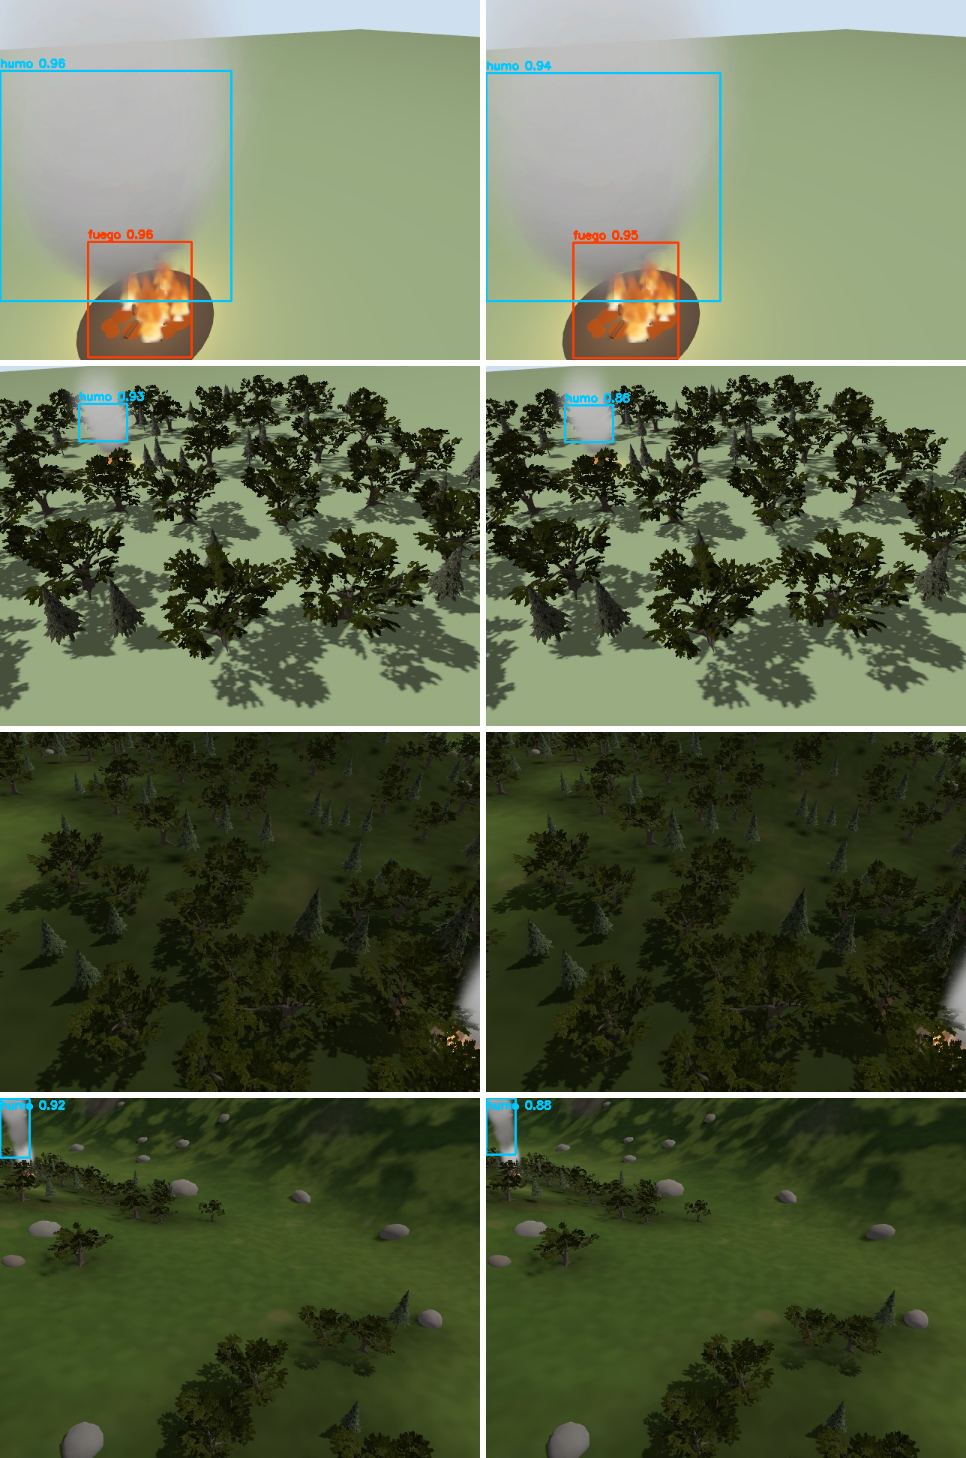
\includegraphics[width=0.92\textwidth]{detecciones.png}
\caption{Detecciones con confianza $\ge 0.25$ en cuatro imágenes de validación.
Izquierda: FuegoNet-n (sin NMS). Derecha: YOLO26n preentrenado de la simulación.}
\label{fig:detecciones}
\end{figure}

